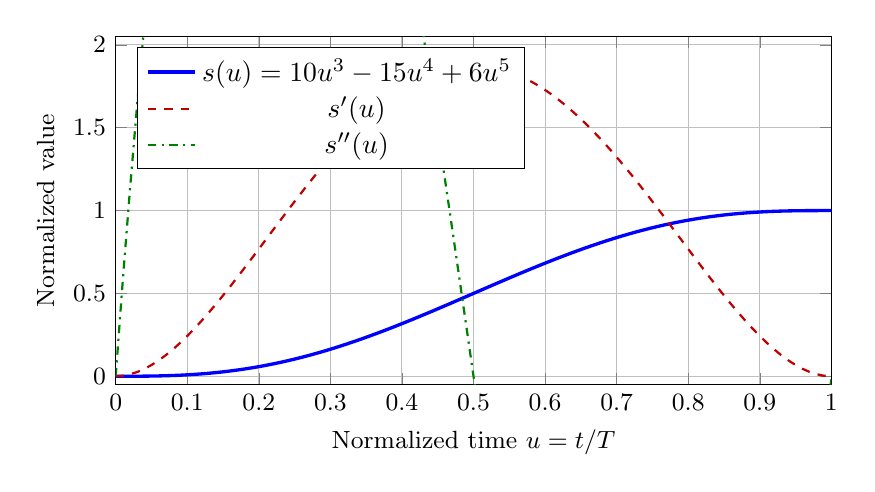
\begin{tikzpicture}
\begin{axis}[
  width=.88\textwidth,height=6cm,
  xlabel={Normalized time $u=t/T$},ylabel={Normalized value},
  xmin=0,xmax=1,ymin=-.05,ymax=2.05,
  grid=both,legend pos=north west,
  tick label style={font=\small},label style={font=\small},
  domain=0:1,samples=100
]
\addplot[blue,very thick] {10*x^3-15*x^4+6*x^5};
\addlegendentry{$s(u)=10u^3-15u^4+6u^5$}
\addplot[red!75!black,thick,dashed] {30*x^2-60*x^3+30*x^4};
\addlegendentry{$s'(u)$}
\addplot[green!50!black,thick,dashdotted] {60*x-180*x^2+120*x^3};
\addlegendentry{$s''(u)$}
\end{axis}
\end{tikzpicture}
